\section{Architettura}

Approfondiamo l'architettura scelta per Easy-Meal, spiegando le scelte
architetturali e i pattern utilizzati per lo sviluppo dell'applicazione partendo
dalla struttura generale del sistema e passando poi ai dettagli implementativi.

\subsection{Architettura di Deployment}

SWEnergy ha deciso di adottare un'architettura a tre livelli (\textit{N-tier
architecture}) per implementare 
Easy-Meal. Questa scelta è stata determinata dalla necessità di costruire una 
web application che permetta agli utenti di accedere al sistema da qualsiasi 
dispositivo connesso a Internet. L'architettura a tre livelli
separa la logica di presentazione dalla logica di business e dal database.

Questo approccio ha permesso al team di sviluppo di lavorare in modo parallelo 
sul \textit{frontend} e sul \textit{backend}, riducendo i tempi di sviluppo e 
facilitando il 
testing del sistema. Inoltre, offre la possibilità di scalare ciascuno 
livello separatamente, in modo da garantire prestazioni ottimali e una 
maggiore flessibilità. Infine, è possibile sostituire l'implementazione di 
uno dei livelli senza dover toccare gli altri, garantendo una maggiore 
manutenibilità del sistema.
In particolare lo sviluppo di Easy-Meal è cominciato partendo dal database,
l'elemento su cui abbiamo posto maggiore enfasi, in quanto è il cuore del
sistema. Successivamente sono stati sviluppati il \textit{backend} e il
\textit{frontend}, in modo da garantire una corretta integrazione tra i
diversi livelli dell'applicazione. SWEnergy ha deciso di utilizzare questa
metodologia, perché le funzionalità messe a disposizione da Easy-Meal al livello
della logica di business sono delle semplici operazioni CRUD, che non richiedono
un'interazione complessa tra i diversi livelli dell'applicazione.

\subsection{Pattern Architetturali}

Easy-Meal è stato sviluppato utilizzando due pattern architetturali:
Model-View-Controller e Dependency Injection. Infatti, SWEnergy ha scelto di
adottare Angular e NestJS, due framework che implementano questi pattern in modo
nativo, garantendo una struttura ben definita e una maggiore manutenibilità del
codice.

\subsubsection{Model-View-Controller}

Il pattern architetturale Model-View-Controller (MVC) è stato utilizzato per
suddividere le responsabilità tra i diversi componenti dell'applicazione. In
particolare, il \textit{model} rappresenta i dati dell'applicazione e fornisce i
metodi di accesso e di modifica di tali dati. NestJS è il framework che
implementa il backend nell'applicativo e fornisce le api di accesso ai dati
di modifica tramite i \textit{controller}. Angular, invece, è il framework che
implementa il frontend e fornisce le interfacce grafiche per la gestione delle
interazione con l'utente, ovvero la \textit{view}. I \textit{component} e i
\textit{controller} sono responsabili di gestire le interazioni tra la 
\textit{view} e il \textit{model},
aggiornando i dati in base alle azioni dell'utente. L'aggiornamento della
visualizzazione dei dati è gestito da Angular, che attraverso il \textit{data
binding} permette di mantenere sincronizzati i dati presenti nel \textit{model}
con la \textit{view}.

\subsubsection{Dependency Injection}

Il pattern Dependency Injection (DI) è stato utilizzato per gestire le
dipendenze tra i diversi componenti dell'applicazione. In particolare, Angular
utilizza la DI per iniettare i servizi all'interno dei componenti, permettendo
di scrivere codice più modulare e manutenibile. NestJS, invece, utilizza la DI
per iniettare i servizi all'interno dei controller, permettendo di separare la
logica di business dalla logica di accesso ai dati. Questo approccio consente di
creare componenti indipendenti e riutilizzabili, facilitando la manutenibilità
dell'applicazione. Infine la divisione in moduli rende il codice facilmente
testabile, in quanto è possibile sostituire i servizi con dei \textit{mock} per
testare i componenti in modo isolato.

\subsection{\textit{Frontend}}

Di seguito sono proposti alcuni diagrammi delle classi per il \textit{frontend}
di Easy-Meal. Poiché la struttura del \textit{frontend} è piuttosto vasta, ma
ridondante, nel senso che il pattern \textit{dependency injection} è applicato
allo stesso modo per tutti i componenti, si è deciso di selezionare alcuni
esempi significativi.

\subsubsection{GenericService}

\begin{figure}[H]
	\centering
	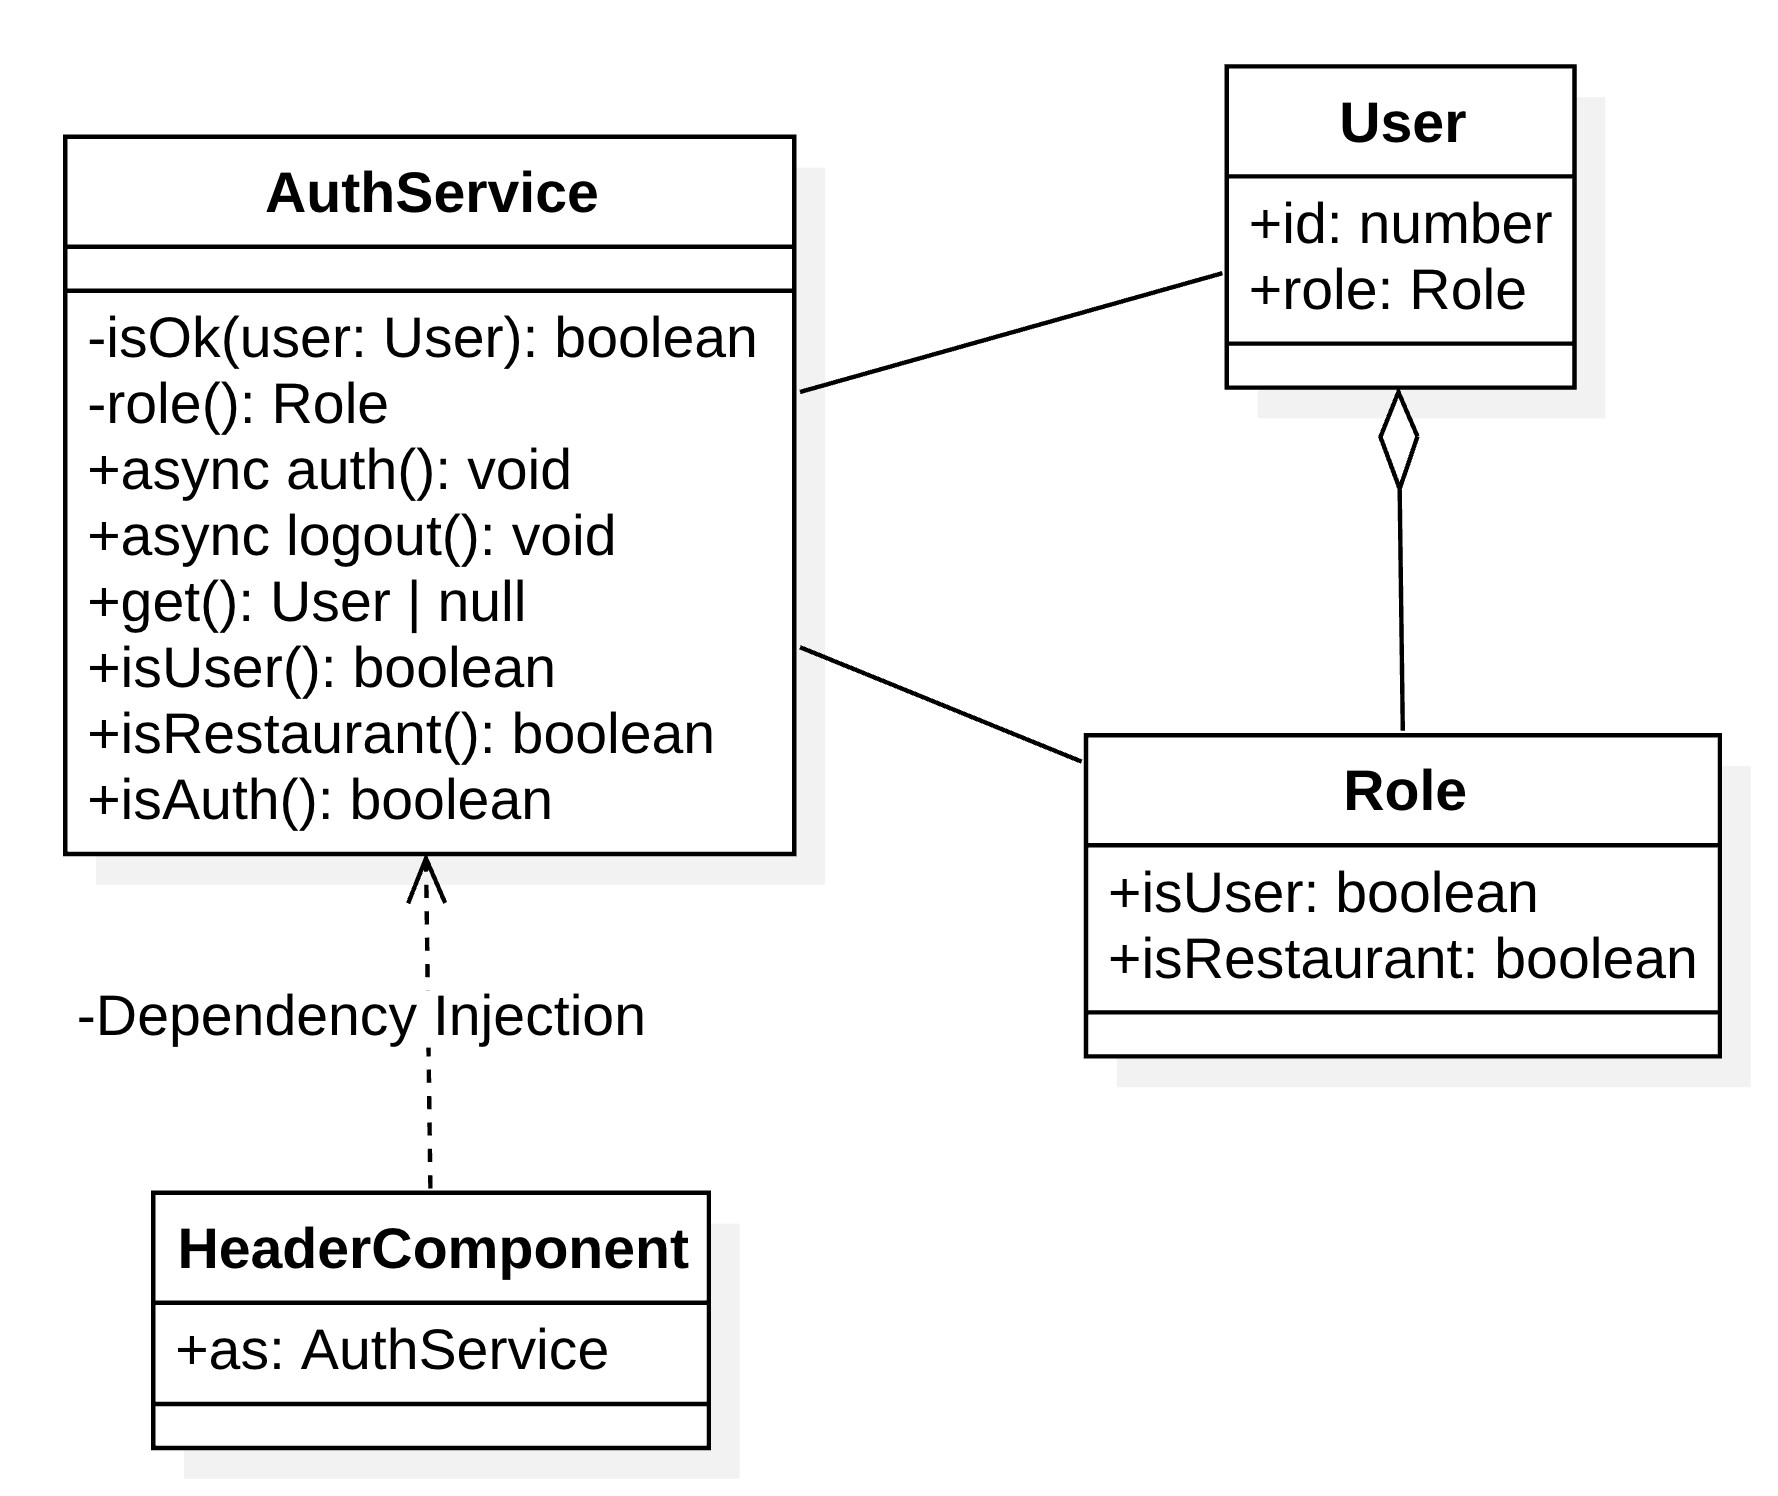
\includegraphics[width=0.5\textwidth]{PB/specifiche-tecniche/auth-service.png}
	\caption{Diagramma delle classi per AuthService}
\end{figure}

In questo caso, viene mostrato come viene iniettato un servizio all'interno di
un componente. Lo \textit{specimen} scelto è il servizio AuthService,
che è responsabile della gestione dell'autenticazione dell'utente. Iniettando
AuthService all'interno del componente HeaderComponent, i metodi pubblici
definiti in AuthService possono essere utilizzati per gestire l'autenticazione
dell'utente. In particolare, HeaderComponent utilizza AuthService per gestire i
link del menu di navigazione in base allo stato di autenticazione e al ruolo 
dell'utente. In questo modo viene favorita la separazione delle responsabilità
e la modularità del codice, rendendo il componente HeaderComponent più
manutenibile e permettendo di riutilizzare AuthService in altri componenti.

\subsubsection{MessageService}

\begin{figure}[H]
	\centering
	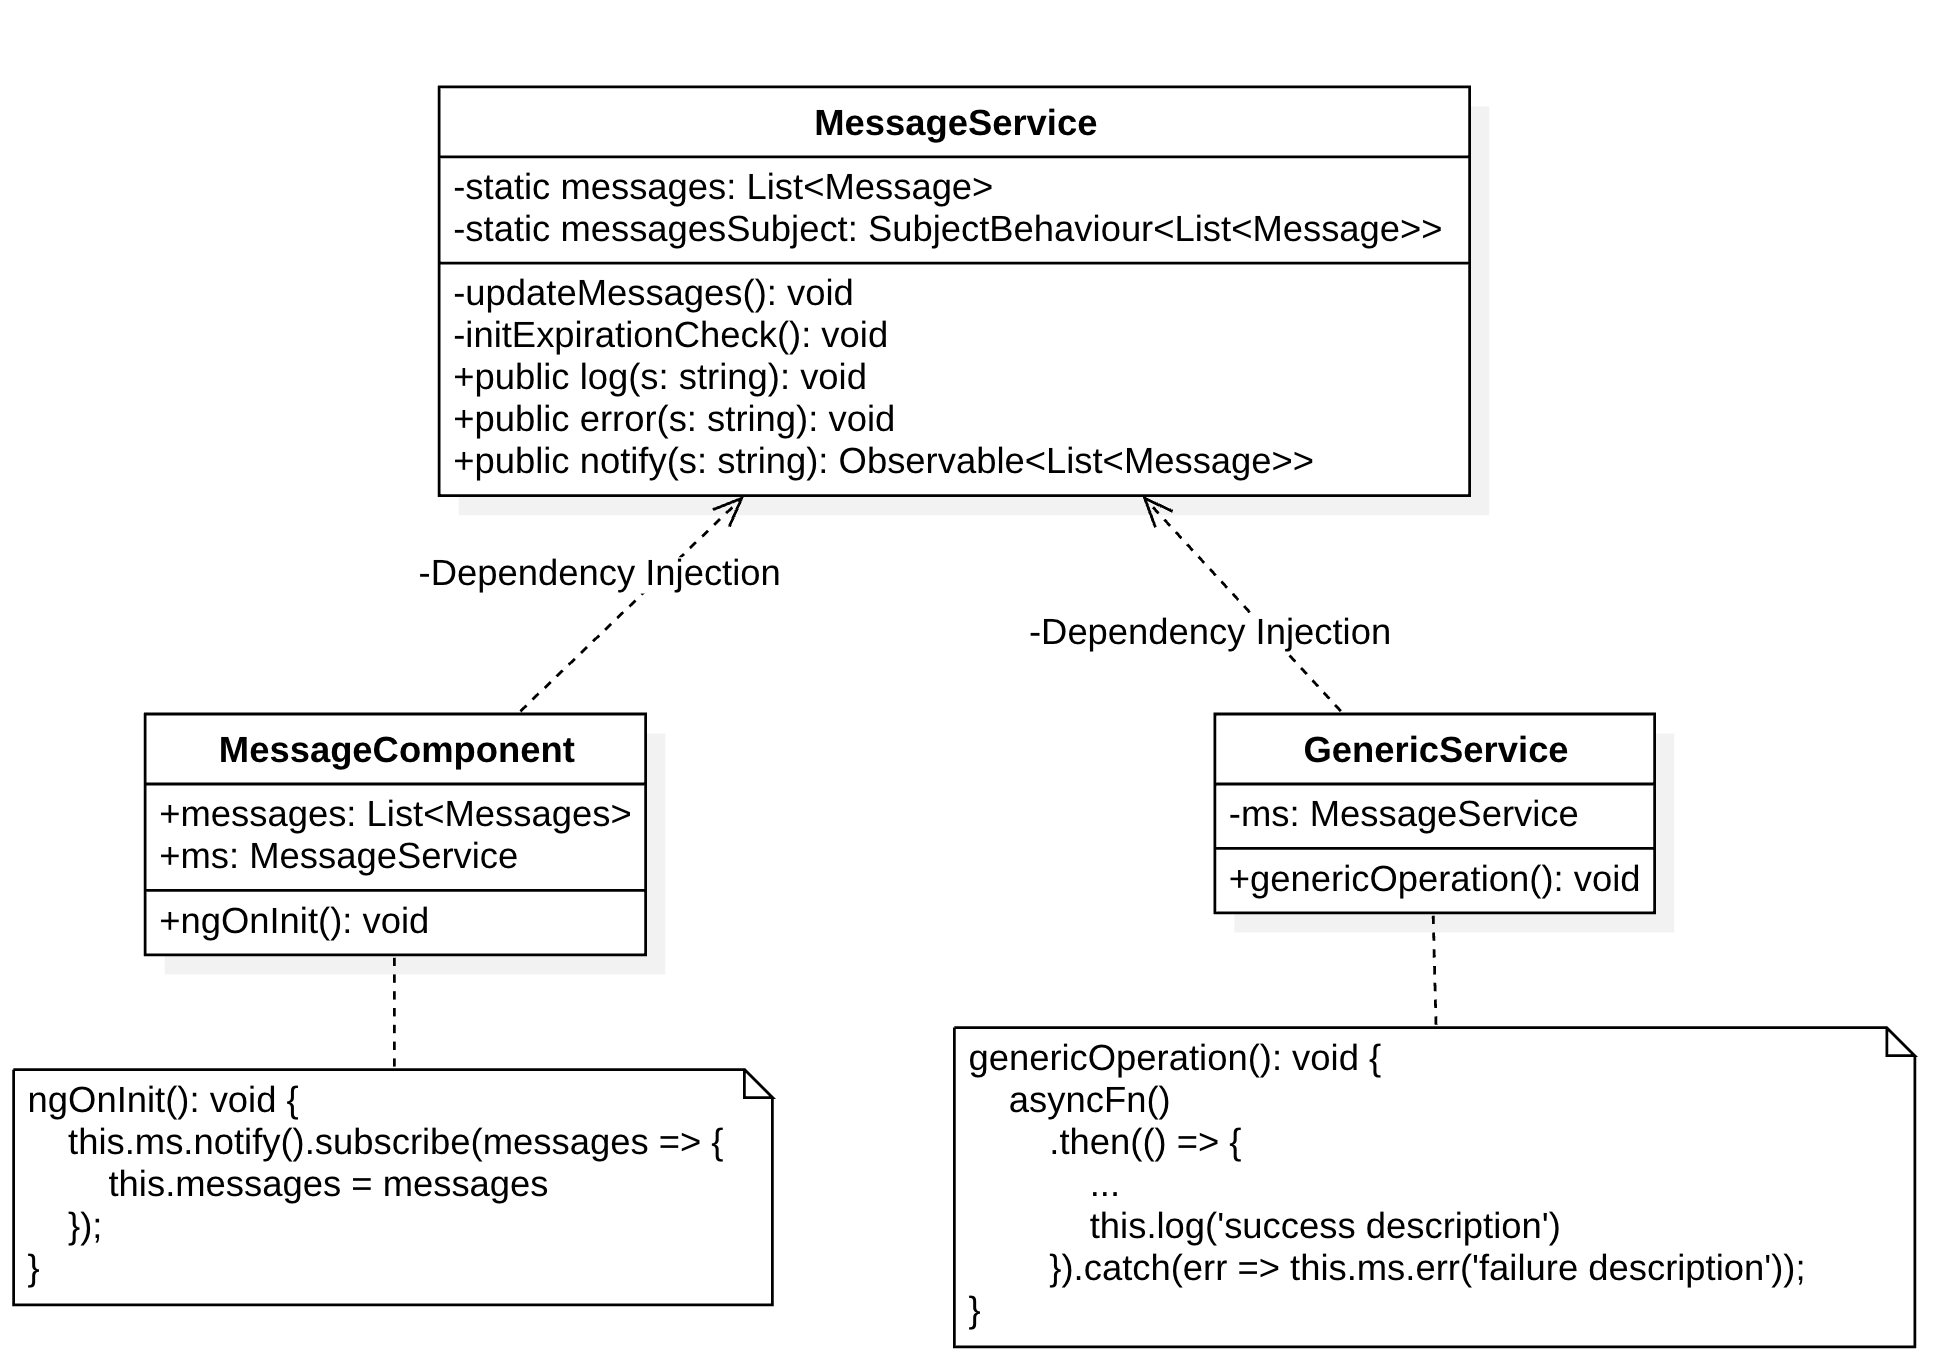
\includegraphics[width=0.8\textwidth]{PB/specifiche-tecniche/message-service.png}
	\caption{Diagramma delle classi per il MessageService}
\end{figure}

La \textit{dependency injection} (DI) in Angular è un \textit{design pattern} che 
consente di fornire dipendenze alle classi in modo automatizzato. In questo 
caso, la classe MessageService viene iniettata sia nella classe 
MessageComponent che nella classe GenericService.
Questo è reso possibile dichiarando MessageService come dipendenza nei 
costruttori delle rispettive classi.
L'annotazione \texttt{@Injectable} viene utilizzata sulla classe MessageService 
per indicare che questa può essere iniettata come dipendenza.\\
MessageService è implementato come singleton in Angular. Un singleton garantisce 
che una sola istanza della classe venga creata e condivisa in tutta 
l'applicazione.
Questo è importante per la gestione centralizzata dello stato e delle operazioni 
comuni, come la gestione dei messaggi.
In Angular, il pattern singleton è implicitamente implementato tramite il 
sistema DI, poiché il servizio è registrato nel \textit{root injector}, 
garantendo una singola istanza.\\
Angular offre un potente meccanismo di \textit{data binding} che consente alla 
vista di aggiornarsi automaticamente quando i dati del modello cambiano.
Nella classe MessageComponent, il metodo \texttt{ngOnInit} utilizza 
l'osservabile restituito da ms.notify() per iscriversi agli aggiornamenti dei 
messaggi.
Quando i messaggi vengono aggiornati nel MessageService, la vista associata a 
MessageComponent si aggiorna automaticamente per riflettere i nuovi dati.
Questo è facilitato dall'utilizzo di Subject o BehaviorSubject in 
MessageService, che emettono nuovi valori quando i messaggi cambiano.\\
In sostanza, in questo modo si utilizza un servizio per condividere dati tra
componenti che non hanno una relazione gerarchica.
